\section{Interactive Interface}\label{sec:5}

This section describes the running prototype as a sequence of interaction patterns.
Each pattern is described by the user's objective, the interaction flow, the system's response, the explanation mechanism, and the control the user retains.
We treat the eight screenshots of \figref{fig:portal} as design artifacts that instantiate the principles of \secref{sec:3}, not as product screenshots.

\leadpara{Overview of the interface surface}
The prototype presents three role-specific portals: a candidate portal for job seekers, an employer portal for recruiters, and an admin/evaluation console.
The candidate and employer portals are the primary surface for the user contribution; the admin/evaluation console supports the inspection and benchmarking discussed in \secref{sec:6} and \secref{sec:7}.
\figref{fig:portal} shows the eight primary interaction states; each is described below.

\begin{figure}[!htbp]
\centering
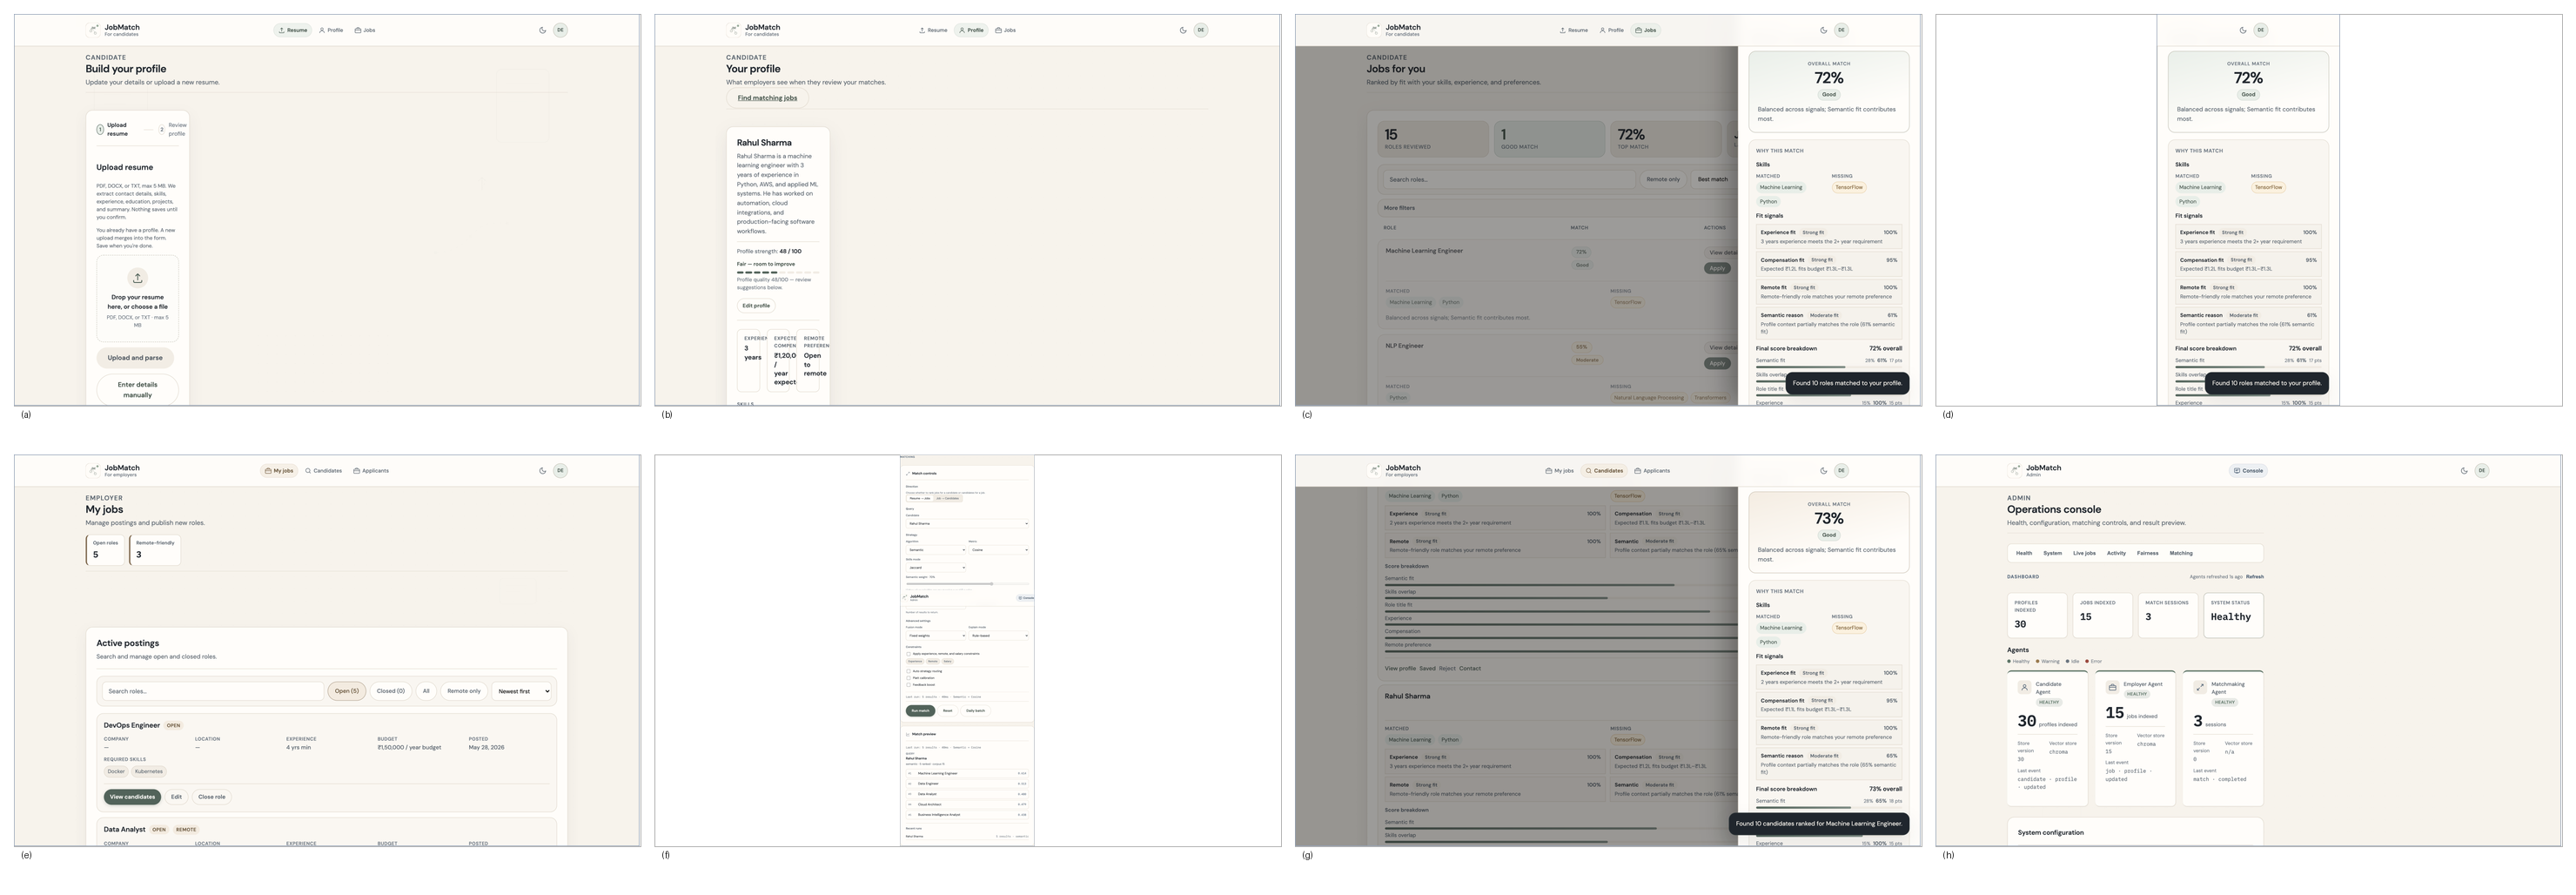
\includegraphics[width=0.95\linewidth]{../figures/Fig10.png}
\caption{The eight primary interaction states of the prototype, ordered as a user would encounter them. Top row (candidate side): (a) resume upload and review; (b) parsed-fields confirmation; (c) match-list view with component-level explanation drawer; (d) counterfactual view showing how a small edit would move the rank. Bottom row (employer side): (e) job-description upload and review; (f) parsed-requirements confirmation; (g) reverse match list with component-level explanation; (h) shortlist panel. The admin/evaluation console is not shown here.}
\label{fig:portal}
\end{figure}

\begin{figure}[!htbp]
\centering
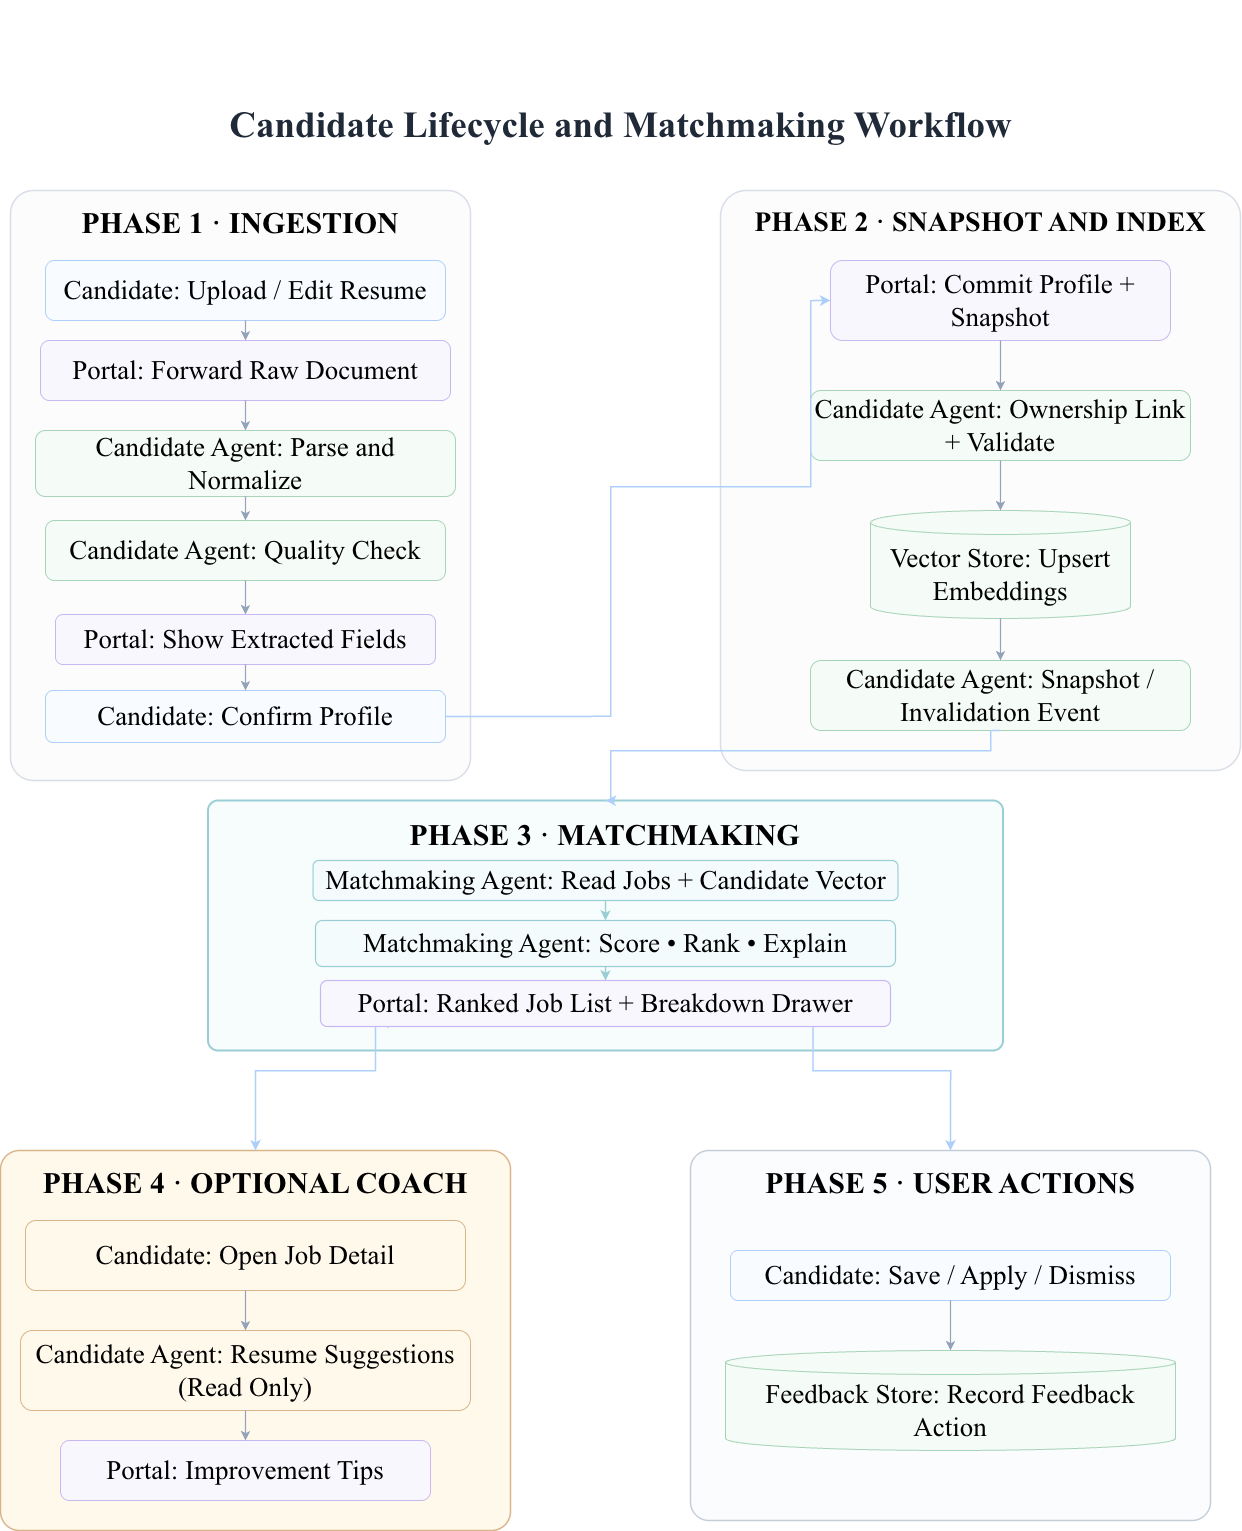
\includegraphics[width=0.95\linewidth]{../figures/Fig6.png}
\caption{Candidate-side lifecycle and matchmaking workflow. The end-to-end candidate journey is: (1) ingestion of the resume and confirmation of the parsed profile, (2) snapshot registration and vector upsert, (3) matchmaking, (4) optional resume-coach feedback (read-only suggestions for the next edit), and (5) user action (save, apply, or dismiss). The matchmaking component is invoked between step 2 and step 5; the optional coach is invoked only on user request and is gated by a per-request budget.}
\label{fig:candidate-lifecycle}
\end{figure}

\leadpara{State (a): candidate resume upload and review}
\emph{User objective.} Upload a resume and have the system extract structured fields without losing the original document.
\emph{Interaction flow.} The user uploads a file; the candidate-side component returns a parsed-fields review form. The user can edit any field and either confirms the snapshot or reverts.
\emph{System response.} A side-by-side view of the original document and the parsed fields, with a confidence flag on each field.
\emph{Explanation mechanism.} Each parsed field carries a small visual marker indicating whether the field was matched against the shared vocabulary directly, was a soft alias, or required user confirmation. This is the transparency property (G1) made tangible.
\emph{User control.} The user can edit any field, toggle the confidence flag, or revert to the original document. No ranking is computed until the user confirms the snapshot.

\leadpara{State (b): candidate parsed-fields confirmation}
\emph{User objective.} Confirm that the parsed fields represent what the user wants the system to compare, or revise them.
\emph{Interaction flow.} The user reviews the parsed fields, edits any field whose value is wrong, and confirms the snapshot.
\emph{System response.} A versioned snapshot identifier and a confirmation receipt. The matchmaking component receives the snapshot identifier and version as an event.
\emph{Explanation mechanism.} Each field has a small icon that links to the original document location from which it was parsed, supporting auditability.
\emph{User control.} Snapshot confirmation is the last point at which the user can revise the parsed fields without re-running the upload; the user can also revert to a previous snapshot from a snapshot-history view.

\leadpara{State (c): candidate match list with component-level explanation}
\emph{User objective.} Read the ranked list of jobs the system recommends, see why each item is ranked where it is, and decide whether to act.
\emph{Interaction flow.} The user opens the match-list view; the matchmaking component returns a ranked list; the user clicks on a list item to open the explanation drawer.
\emph{System response.} A ranked list with a component-level reason for each item, a calibrated confidence value, and an action menu.
\emph{Explanation mechanism.} The explanation drawer shows the contribution of each composite channel to the item's position, a small text rationale generated from the channel contributions, and a counterfactual preview.
\emph{User control.} The user can save the item, dismiss the item, open the counterfactual view, or close the drawer without acting. Apply is a separate, deliberate action and is the only operation that triggers a side effect outside the user's own state.

\leadpara{State (d): candidate counterfactual view}
\emph{User objective.} Understand which small change to a snapshot field would move a list item up or down the ranking.
\emph{Interaction flow.} The user selects a list item and opens the counterfactual view; the matchmaking component returns a small set of proposed edits; the user reads the predicted effect.
\emph{System response.} A list of proposed edits, each annotated with the predicted change in rank and the predicted change in score.
\emph{Explanation mechanism.} Each proposed edit shows the field that would change, the new value, and the resulting change in the composite score.
\emph{User control.} The user can apply a proposed edit (which routes the new field back to the candidate-side component for confirmation), copy it as a note, or close the view.

\leadpara{State (e): employer job-description upload and review}
\emph{User objective.} Upload a job description and have the system extract required and preferred skills, experience bounds, compensation, and remote policy.
\emph{Interaction flow.} Mirrors the candidate upload flow; the recruiter reviews the parsed requirements and confirms.
\emph{System response.} A review form distinguishing required from preferred requirements, with a confidence flag on each.
\emph{Explanation mechanism.} Each requirement carries a marker indicating how it was detected (direct, soft alias, or user-confirmed).
\emph{User control.} The recruiter can toggle any requirement between required and preferred, edit any value, and revert to the original description.

\leadpara{State (f): employer parsed-requirements confirmation}
\emph{User objective.} Confirm the requirements that the system will use to rank candidates.
\emph{Interaction flow.} The recruiter reviews the parsed requirements, edits any value, and confirms the snapshot.
\emph{System response.} A versioned snapshot identifier and a confirmation receipt; the matchmaking component receives the snapshot as an event.
\emph{Explanation mechanism.} A small visual indicator on each requirement shows whether the requirement currently constrains the ranking.
\emph{User control.} Snapshot confirmation is the last point at which the recruiter can revise the requirements.

\leadpara{State (g): employer reverse match list}
\emph{User objective.} Read the ranked list of candidates the system recommends for a posting, see why each candidate is ranked where they are, and decide whether to act.
\emph{Interaction flow.} Mirrors the candidate-side match list; the recruiter clicks an item to open the explanation drawer.
\emph{System response.} A ranked list with component-level reasons, a calibrated confidence value, and a shortlist or contact action menu.
\emph{Explanation mechanism.} The explanation drawer shows the candidate's parsed fields, the contribution of each composite channel, and a short text rationale.
\emph{User control.} Shortlist and contact are separate, deliberate actions; the recruiter can also dismiss a candidate or open the counterfactual view.

\leadpara{State (h): employer shortlist panel}
\emph{User objective.} Review the candidates the recruiter has shortlisted, and confirm or revise the decisions.
\emph{Interaction flow.} The recruiter opens the shortlist panel; the system returns the current shortlist with the rationale that produced it.
\emph{System response.} A list of shortlist items with their original explanation, a confidence value, and a status flag.
\emph{Explanation mechanism.} Each item links back to the match-list view and the explanation drawer that produced the shortlist.
\emph{User control.} The recruiter can remove an item from the shortlist, contact a candidate, or revisit the original explanation.

\leadpara{What the interface is not}
The prototype is not a deployment and is not optimized for production-scale workloads.
It is a research artifact designed to make the principles of \secref{sec:3} concrete and to support the evaluation in \secref{sec:6} and \secref{sec:7}.
The interface does not attempt to be a polished consumer product; it is a controlled surface in which every screen corresponds to a stated design choice and every consequential action is a deliberate user gesture.
